\RequirePackage{plautopatch}
\RequirePackage[l2tabu,orthodox]{nag}
\documentclass[platex,dvipdfmx,10pt,twoside,a4paper,jis2004]{jsarticle}
\usepackage[top=4cm,bottom=3cm,left=2cm,right=2cm]{geometry}

\usepackage[deluxe]{otf}
\usepackage[T1]{fontenc}
\usepackage{lmodern}
\usepackage{textcomp}
\usepackage[geometry,electronic,weather,clock,alpine,misc]{ifsym}
\usepackage{xcolor}
\renewcommand{\sfdefault}{cmr}

\usepackage{ascmac}
\usepackage{fancybox}
\usepackage{tcolorbox}
\usepackage{ulem}
\usepackage{pxrubrica}
\usepackage{seqsplit}
\usepackage{enumitem}

\usepackage{amssymb,amsmath,amsfonts}
\usepackage{physics}
\usepackage[version=4]{mhchem}
\usepackage{bm}

\usepackage{graphicx}
\usepackage{float}
\usepackage{booktabs}
\usepackage{longtable}
\usepackage{tabularx}
\usepackage{colortbl}
\usepackage{multicol}
\usepackage{multirow}
\usepackage{dcolumn}
\usepackage{caption}
\captionsetup[figure]{labelformat=empty}
\captionsetup[table]{labelformat=empty}

\usepackage[colorlinks=true,linkcolor=blue,urlcolor=cyan,citecolor=red]{hyperref}

\usepackage{titlesec}
\titleformat{\section}{\LARGE\bfseries}{\normalfont\thesection}{1em}{}
\titleformat{\subsection}{\Large\bfseries}{\normalfont\thesection}{1em}{}

\title{TES IV Curve Analysis Results}
\author{}
\vspace{-5zw}
\date{\today}

\begin{document}
\maketitle
本解析では,TESの$I-V$測定で得られたデータから,TESカロリメータの諸パラメータを決定する。
\par
測定では,バイアス電流$I_{\rm bias}$に対する出力電圧$V_{\rm out}$を調べる。これについて,まずは電流電圧変換係数$\Xi$を用いてTESの$I-V$特性を得る。さらに,異なる熱浴温度$T_{\rm bath}$における$I-V$特性を求めることで,フィッティングにより熱伝導率$G$や温度依存性のべき定数$n$,TESの温度$T_{\rm TES}$が決定できる。また,TESの$R-T$特性を調べることで転移温度$T_{\rm c}$がわかり,温度感度$\alpha$が計算できる。

\section*{Fitting Parameters}
フィッティング結果のパラメータをまとめる。
\begin{itemize}
    \item \textbf{Tc (TES Temperature)}: $0.146\ {\rm K}$
    \item \textbf{G0 (Thermal Conductivity at 1K)}: $171.490\ {\rm nW/K}$
    \item \textbf{n (Power Constant)}: $4.00$
    \item \textbf{Chi-squared (Minimum)}: $0.66$
\end{itemize}
\clearpage

\section*{Plot Results}
\subsection*{IVtes\_IVproperty}
TESに流れる電流$I_{\rm TES}$とTESの両端にかかる電圧$V_{\rm TES}$の関係
\[
V_{\rm TES} = \frac{V_{\rm TES}}{R_{\rm TES}}
\]
をプロットする。$R_{\rm TES}$はTESの抵抗である。このとき,$I_{\rm TES}$は出力電圧$V_{\rm out}$と電流電圧変換係数$\Xi$を用いて
\[
I_{\rm TES} \simeq \frac{1}{\Xi}V_{\rm out}
\]
で求められる。$\Xi$は,SQUIDの入力コイル相互インダクタンス$M_{\rm in}$,フィードバックコイル相互インダクタンス$M_{\rm FB}$,フィードバック抵抗値$R_{\rm FB}$により
\[
\Xi = \frac{M_{\rm in}}{M_{\rm FB}}R_{\rm FB}
\]
で表される係数。また,$R_{\rm TES}$は測定バイアス電流$I_{\rm bias}$シャント抵抗$R_{\rm sh}$を用いて
\[
R_{\rm TES} = \left(\frac{I_{\rm bias}}{I_{\rm TES}}-1\right)R_{\rm sh}
\]
で書ける。\\ 左上図は各熱浴温度$T_{\rm bath}$に対する測定結果の$V_{\rm out}$と$I_{\rm bias}$の関係をプロットしたもので,右上図はそのグラフを超伝導転移端付近で拡大したものである。
また,左下図は各熱浴温度$T_{\rm bath}$に対する計算結果の$V_{\rm TES}$と$I_{\rm TES}$の関係をプロットしたもので,右下図はそのグラフを超伝導転移端付近で拡大したものである。
\begin{figure}[H]
    \centering
    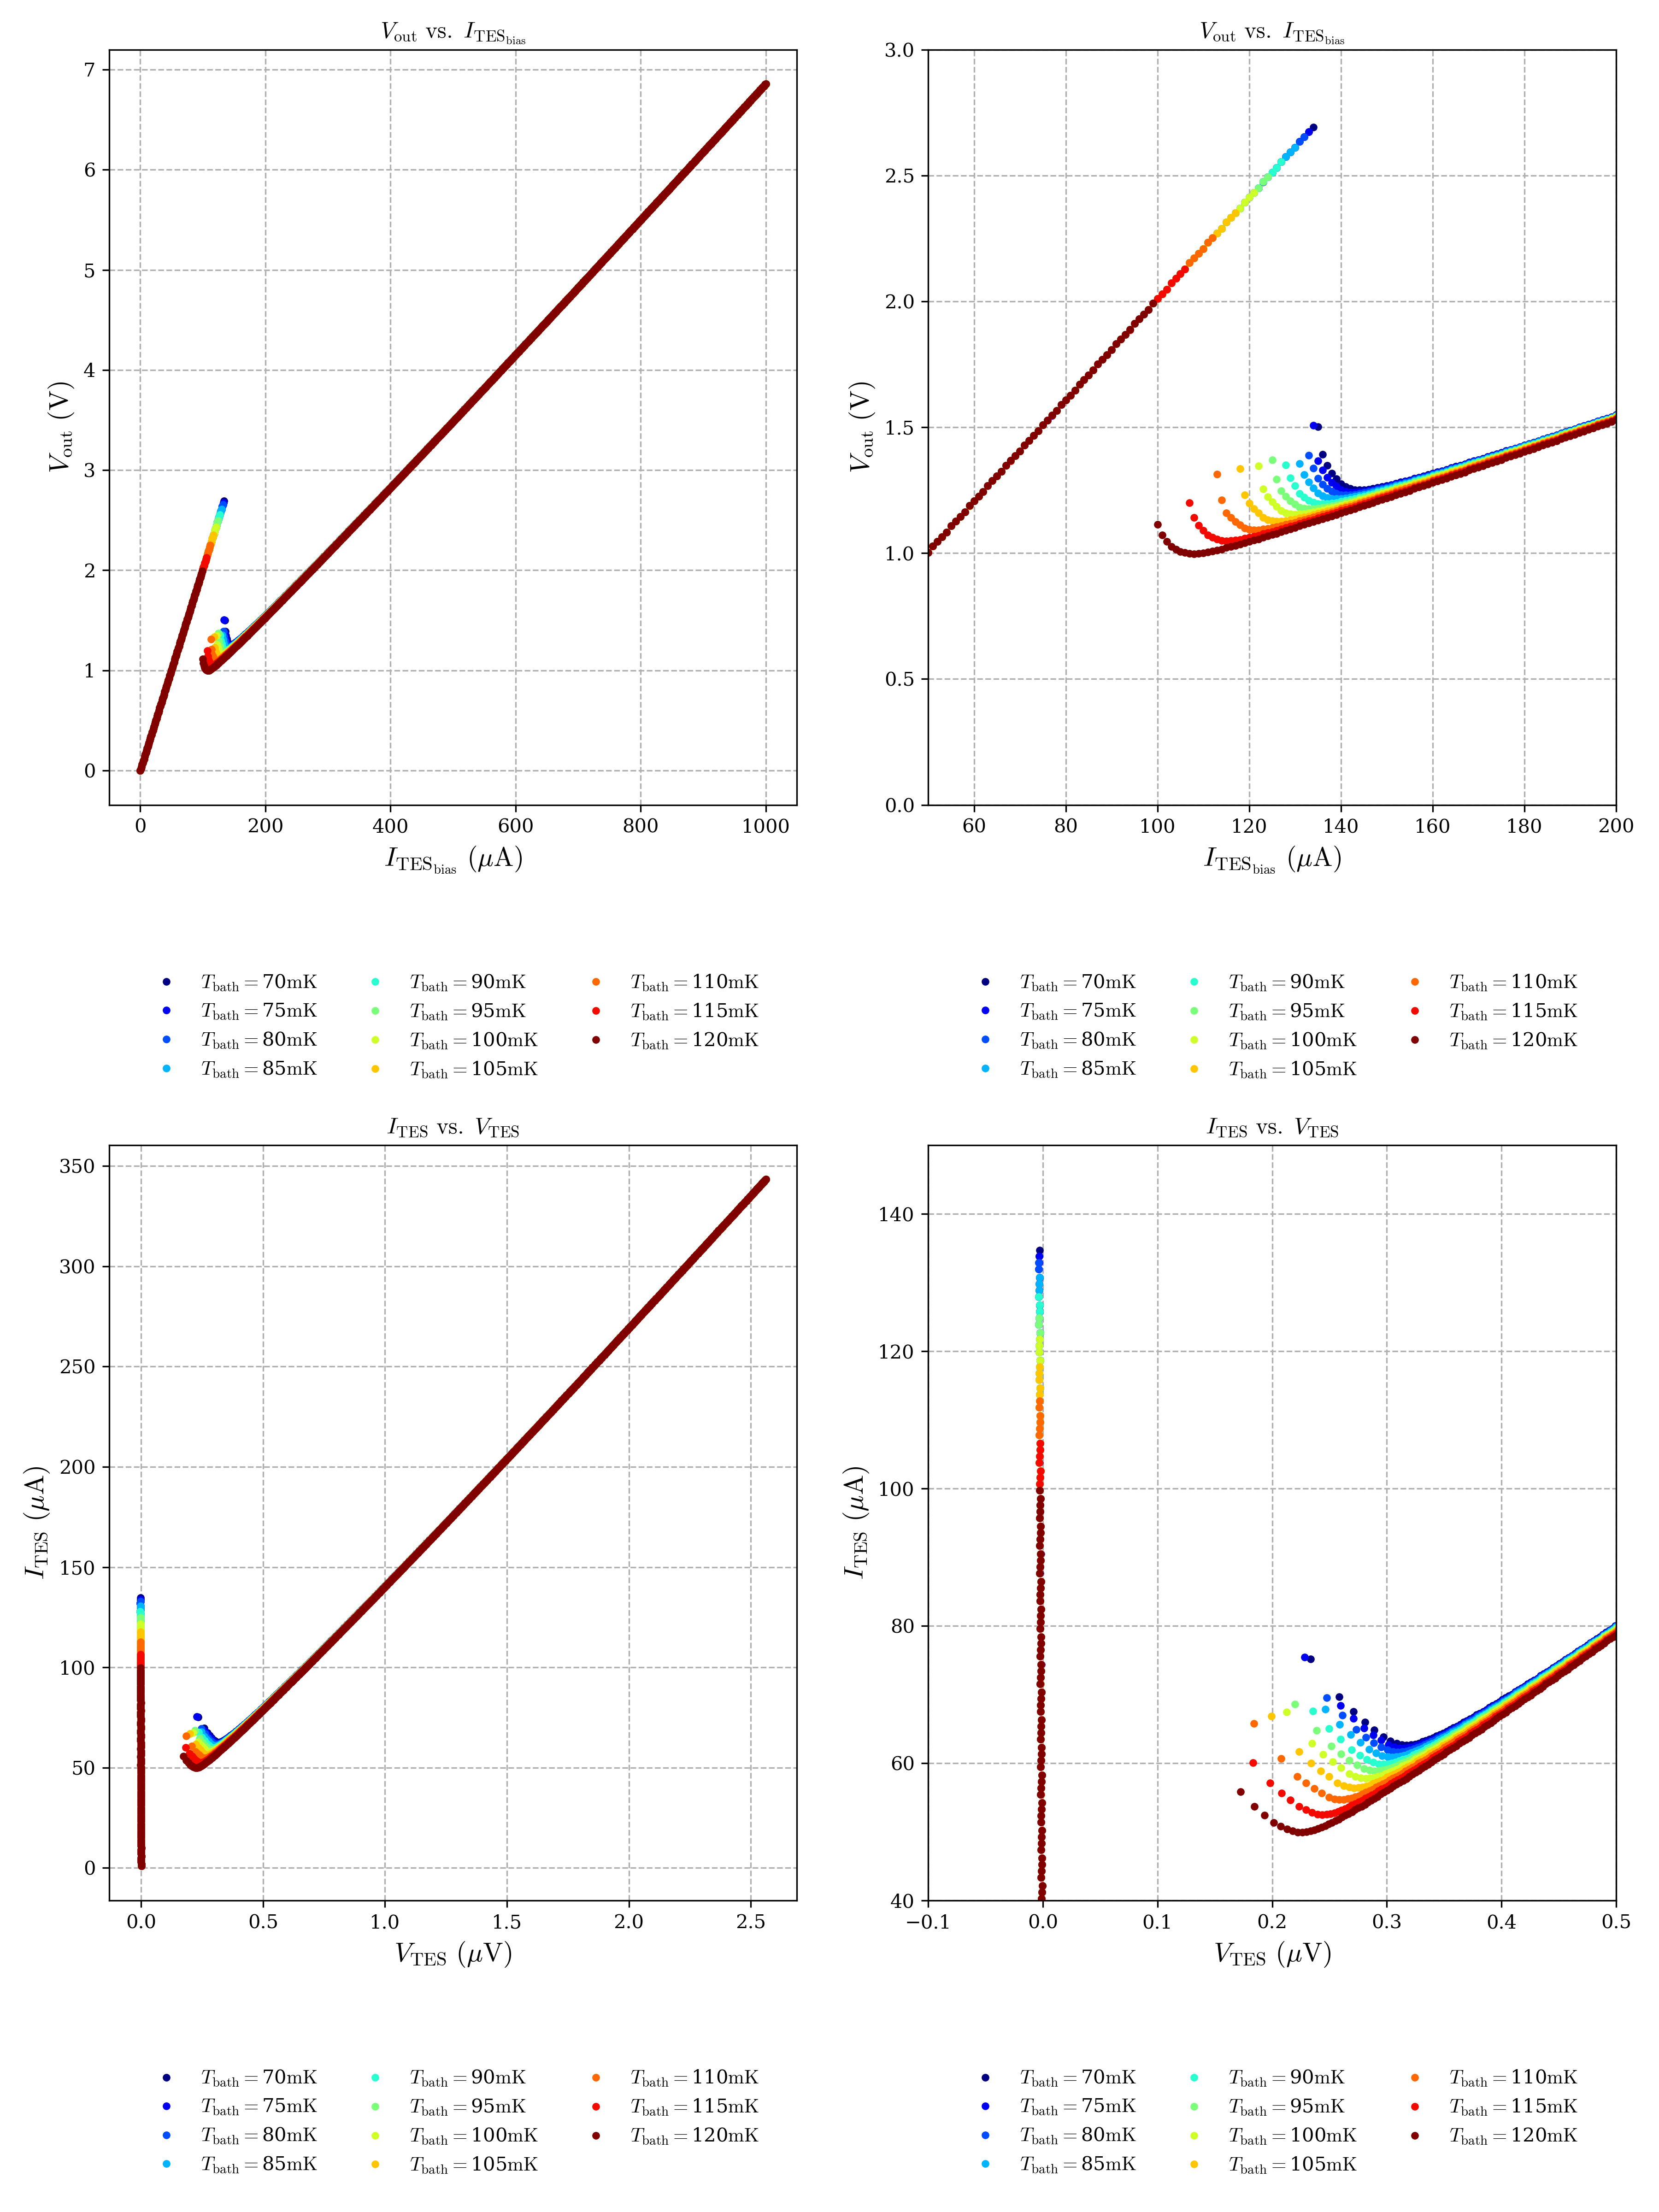
\includegraphics[width=0.8\textwidth]{IVtes_IVproperty.png}
    \label{fig:IVtesIVproperty}
\end{figure}
\clearpage

\subsection*{IVtes\_PRproperty}
TESの抵抗$R_{\rm TES }$とTESのJoule発熱$P_{\rm TES}$の関係をプロットする。ここでの$R_{\rm TES}$は,正規化したTESの抵抗とする。
\\ 左図は$R_{\rm TES }$と$P_{\rm TES}$の関係をプロットしたもので,右図はそのグラフを超伝導転移端付近で拡大したものである。
\begin{figure}[H]
    \centering
    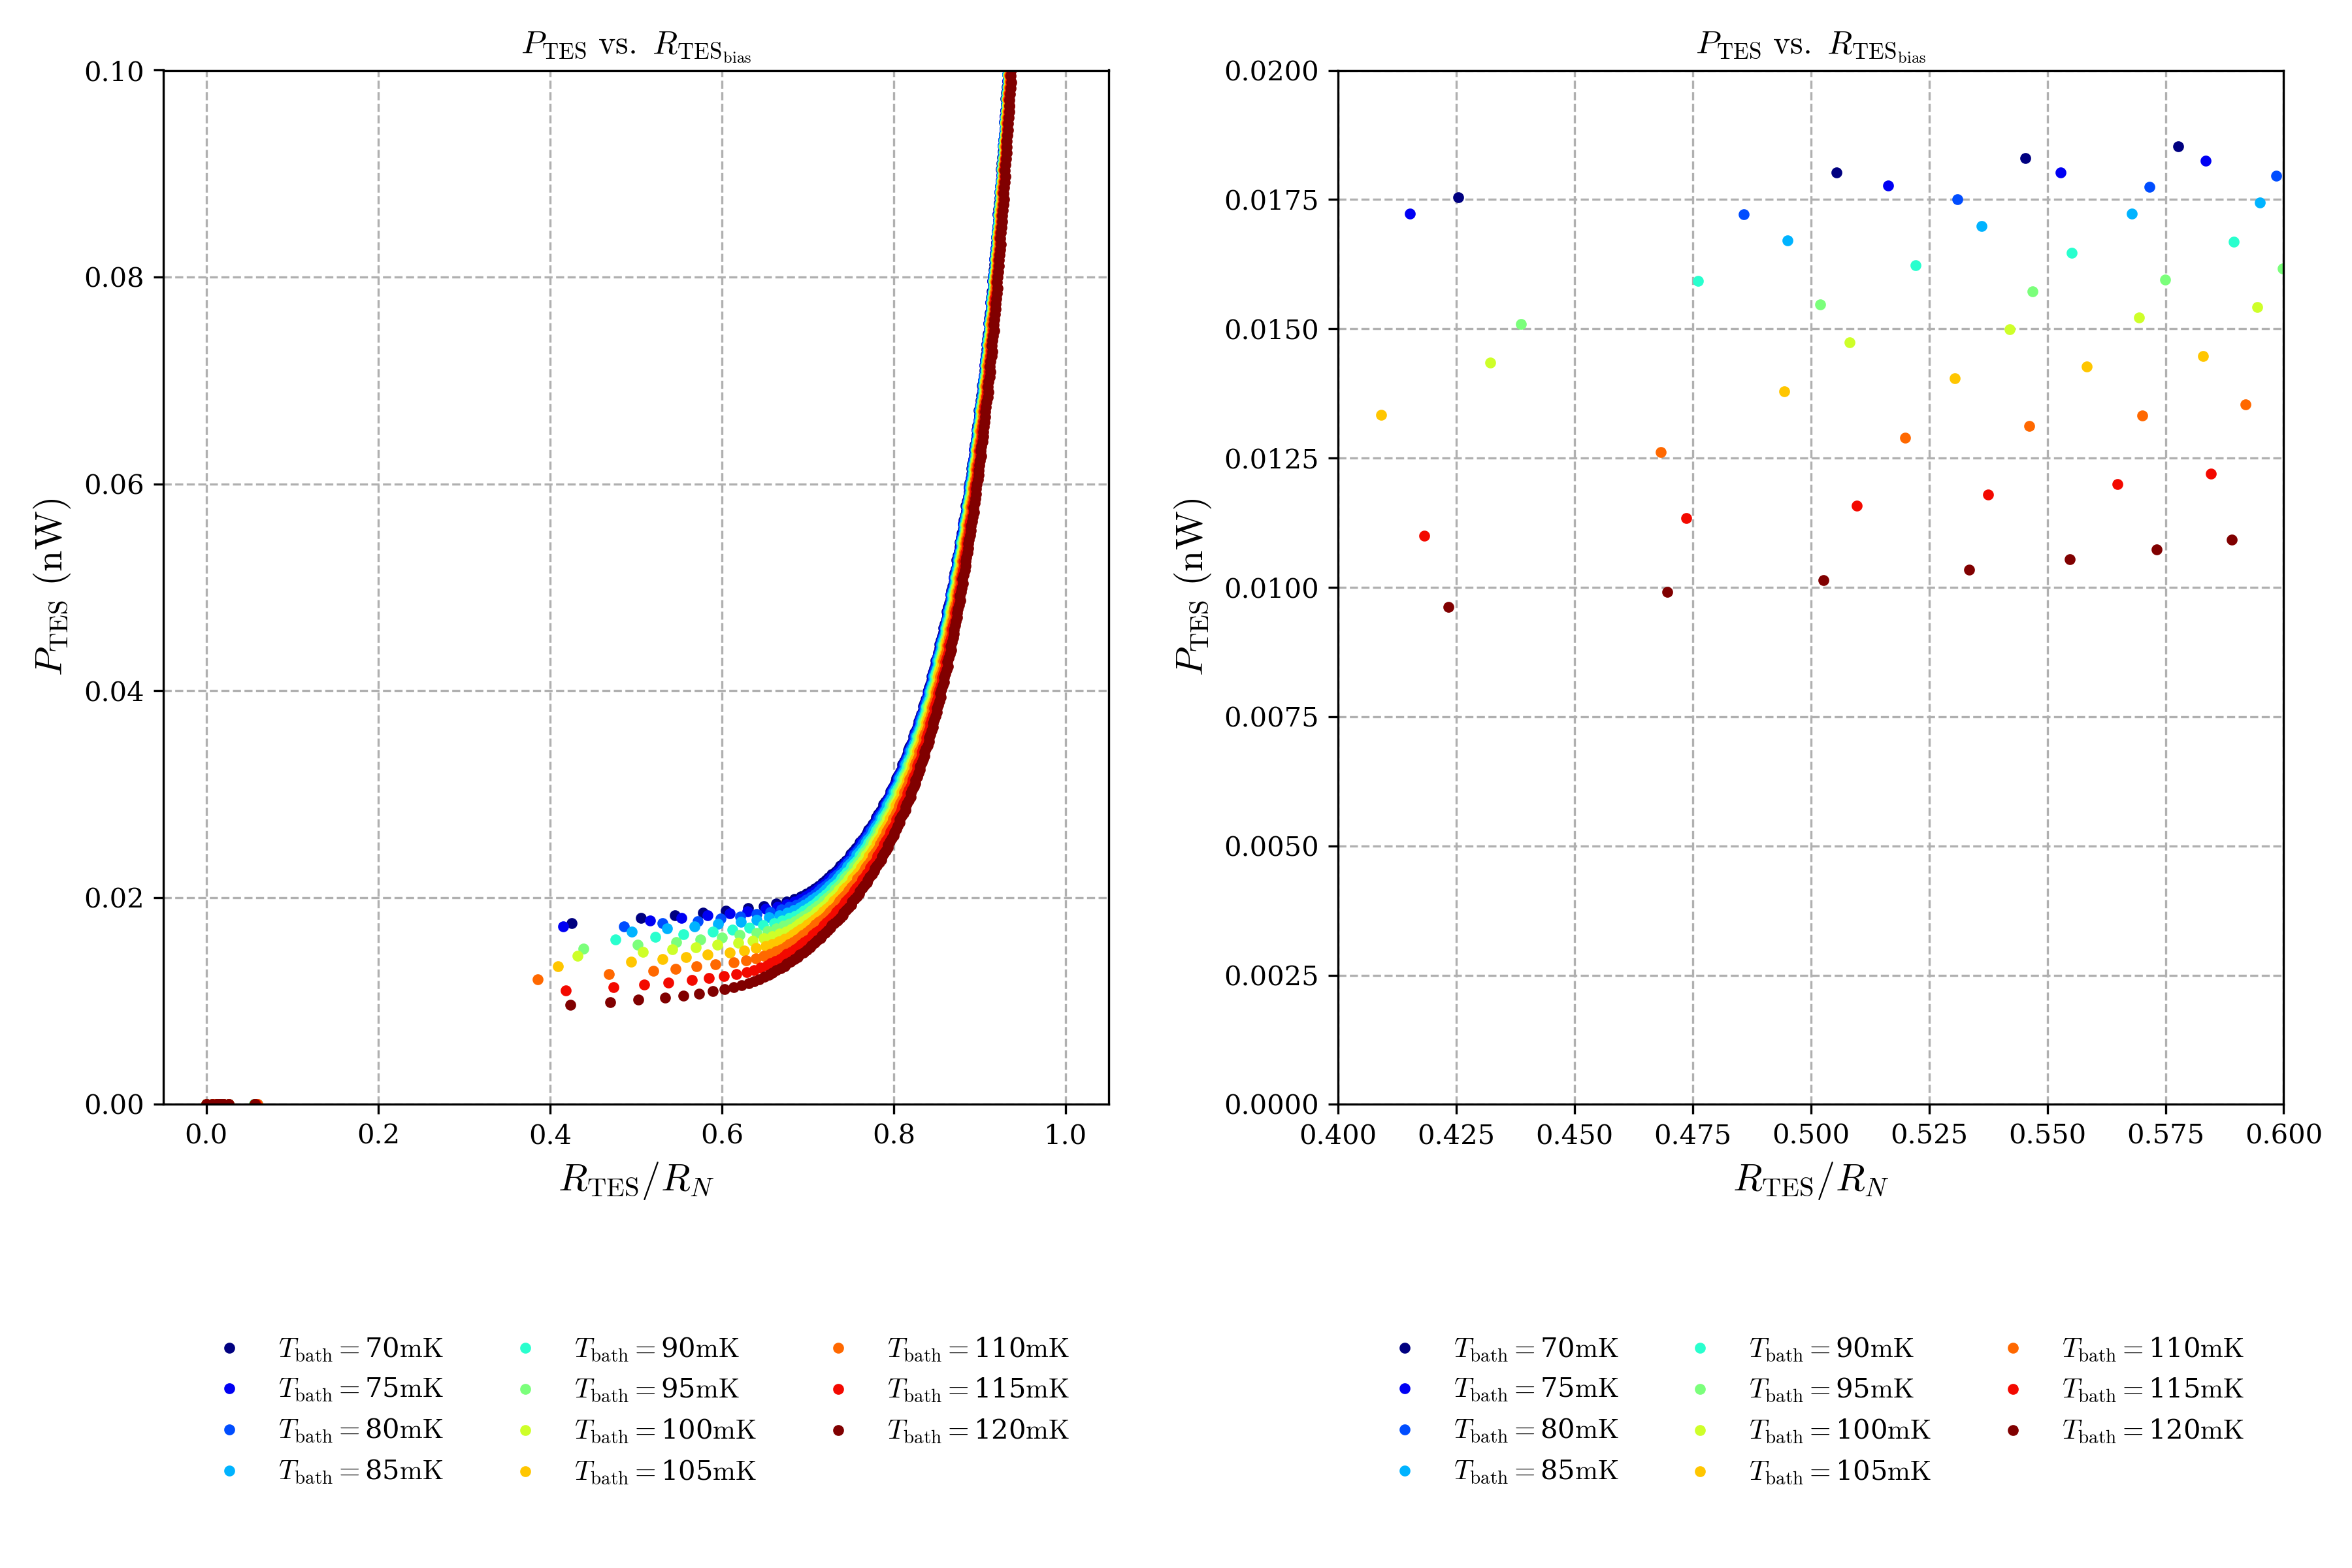
\includegraphics[width=0.8\textwidth]{IVtes_PRproperty.png}
    \label{fig:IVtesPRproperty}
\end{figure}
\clearpage

\subsection*{IVtes\_fitting}
TESのJoule発熱$P_{\rm TES}$と熱浴温度$T_{\rm bath}$の関係
\[
P_{\rm TES} = \frac{G_0}{n}(T_{\rm TES}^n - T_{\rm bath}^n)
\]
をフィッティングする。$P_{\rm TES}$は,PR特性グラフからTESの超伝導転移端の$P_{\rm TES}$(Joule発熱が一定の領域)を平均した代表値を使う。
フィッティングにより,TESの超伝導転移端$T_{\rm c}$,熱浴温度が$1\ {\rm K}$のときの熱伝導度$G_0$,べき定数$n$のそれぞれの最適値が得られる。
\\ 図は$P_{\rm TES}$(誤差付き)と$T_{\rm bath}$の関係をプロットしたものと,そのフィッティング結果。$P_{\rm TES}$の誤差は不偏標準偏差で計算した。

\begin{figure}[H]
    \centering
    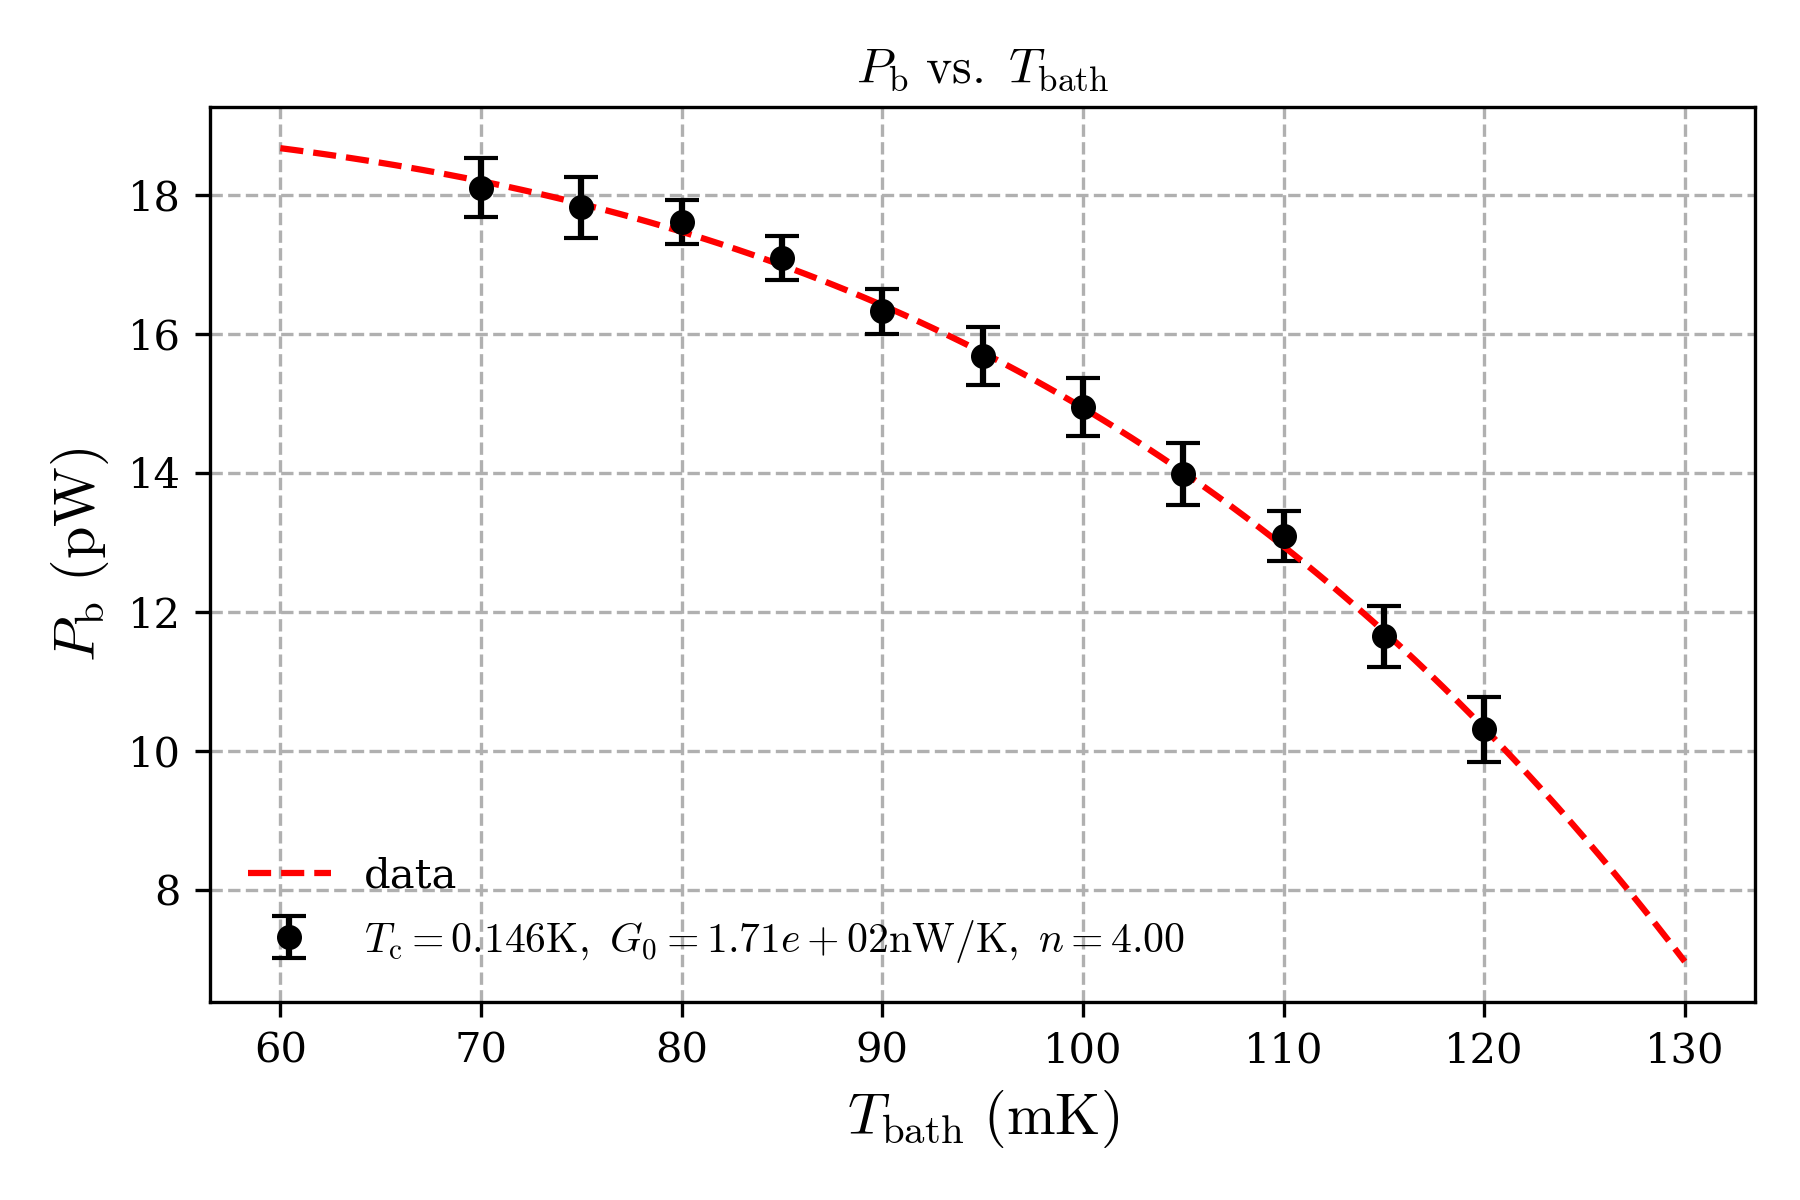
\includegraphics[width=0.8\textwidth]{IVtes_fitting.png}
    \label{fig:IVtesfitting}
\end{figure}
\clearpage

\subsection*{IVtes\_RTproperty}
TESの抵抗$R_{\rm TES }$とTESの温度$T_{\rm TES}$の関係をプロットする。$T_{\rm TES}$は,フィッティング関数を逆算して
\[
T_{\rm TES} = \left(T_{\rm bath}^n + \frac{n\cdot P_{\rm TES}}{G_0}\right)^{1/n}
\]
で計算できる。\\ 図は$R_{\rm TES }$と$T_{\rm TES}$の関係をプロットしたものである。
\begin{figure}[H]
    \centering
    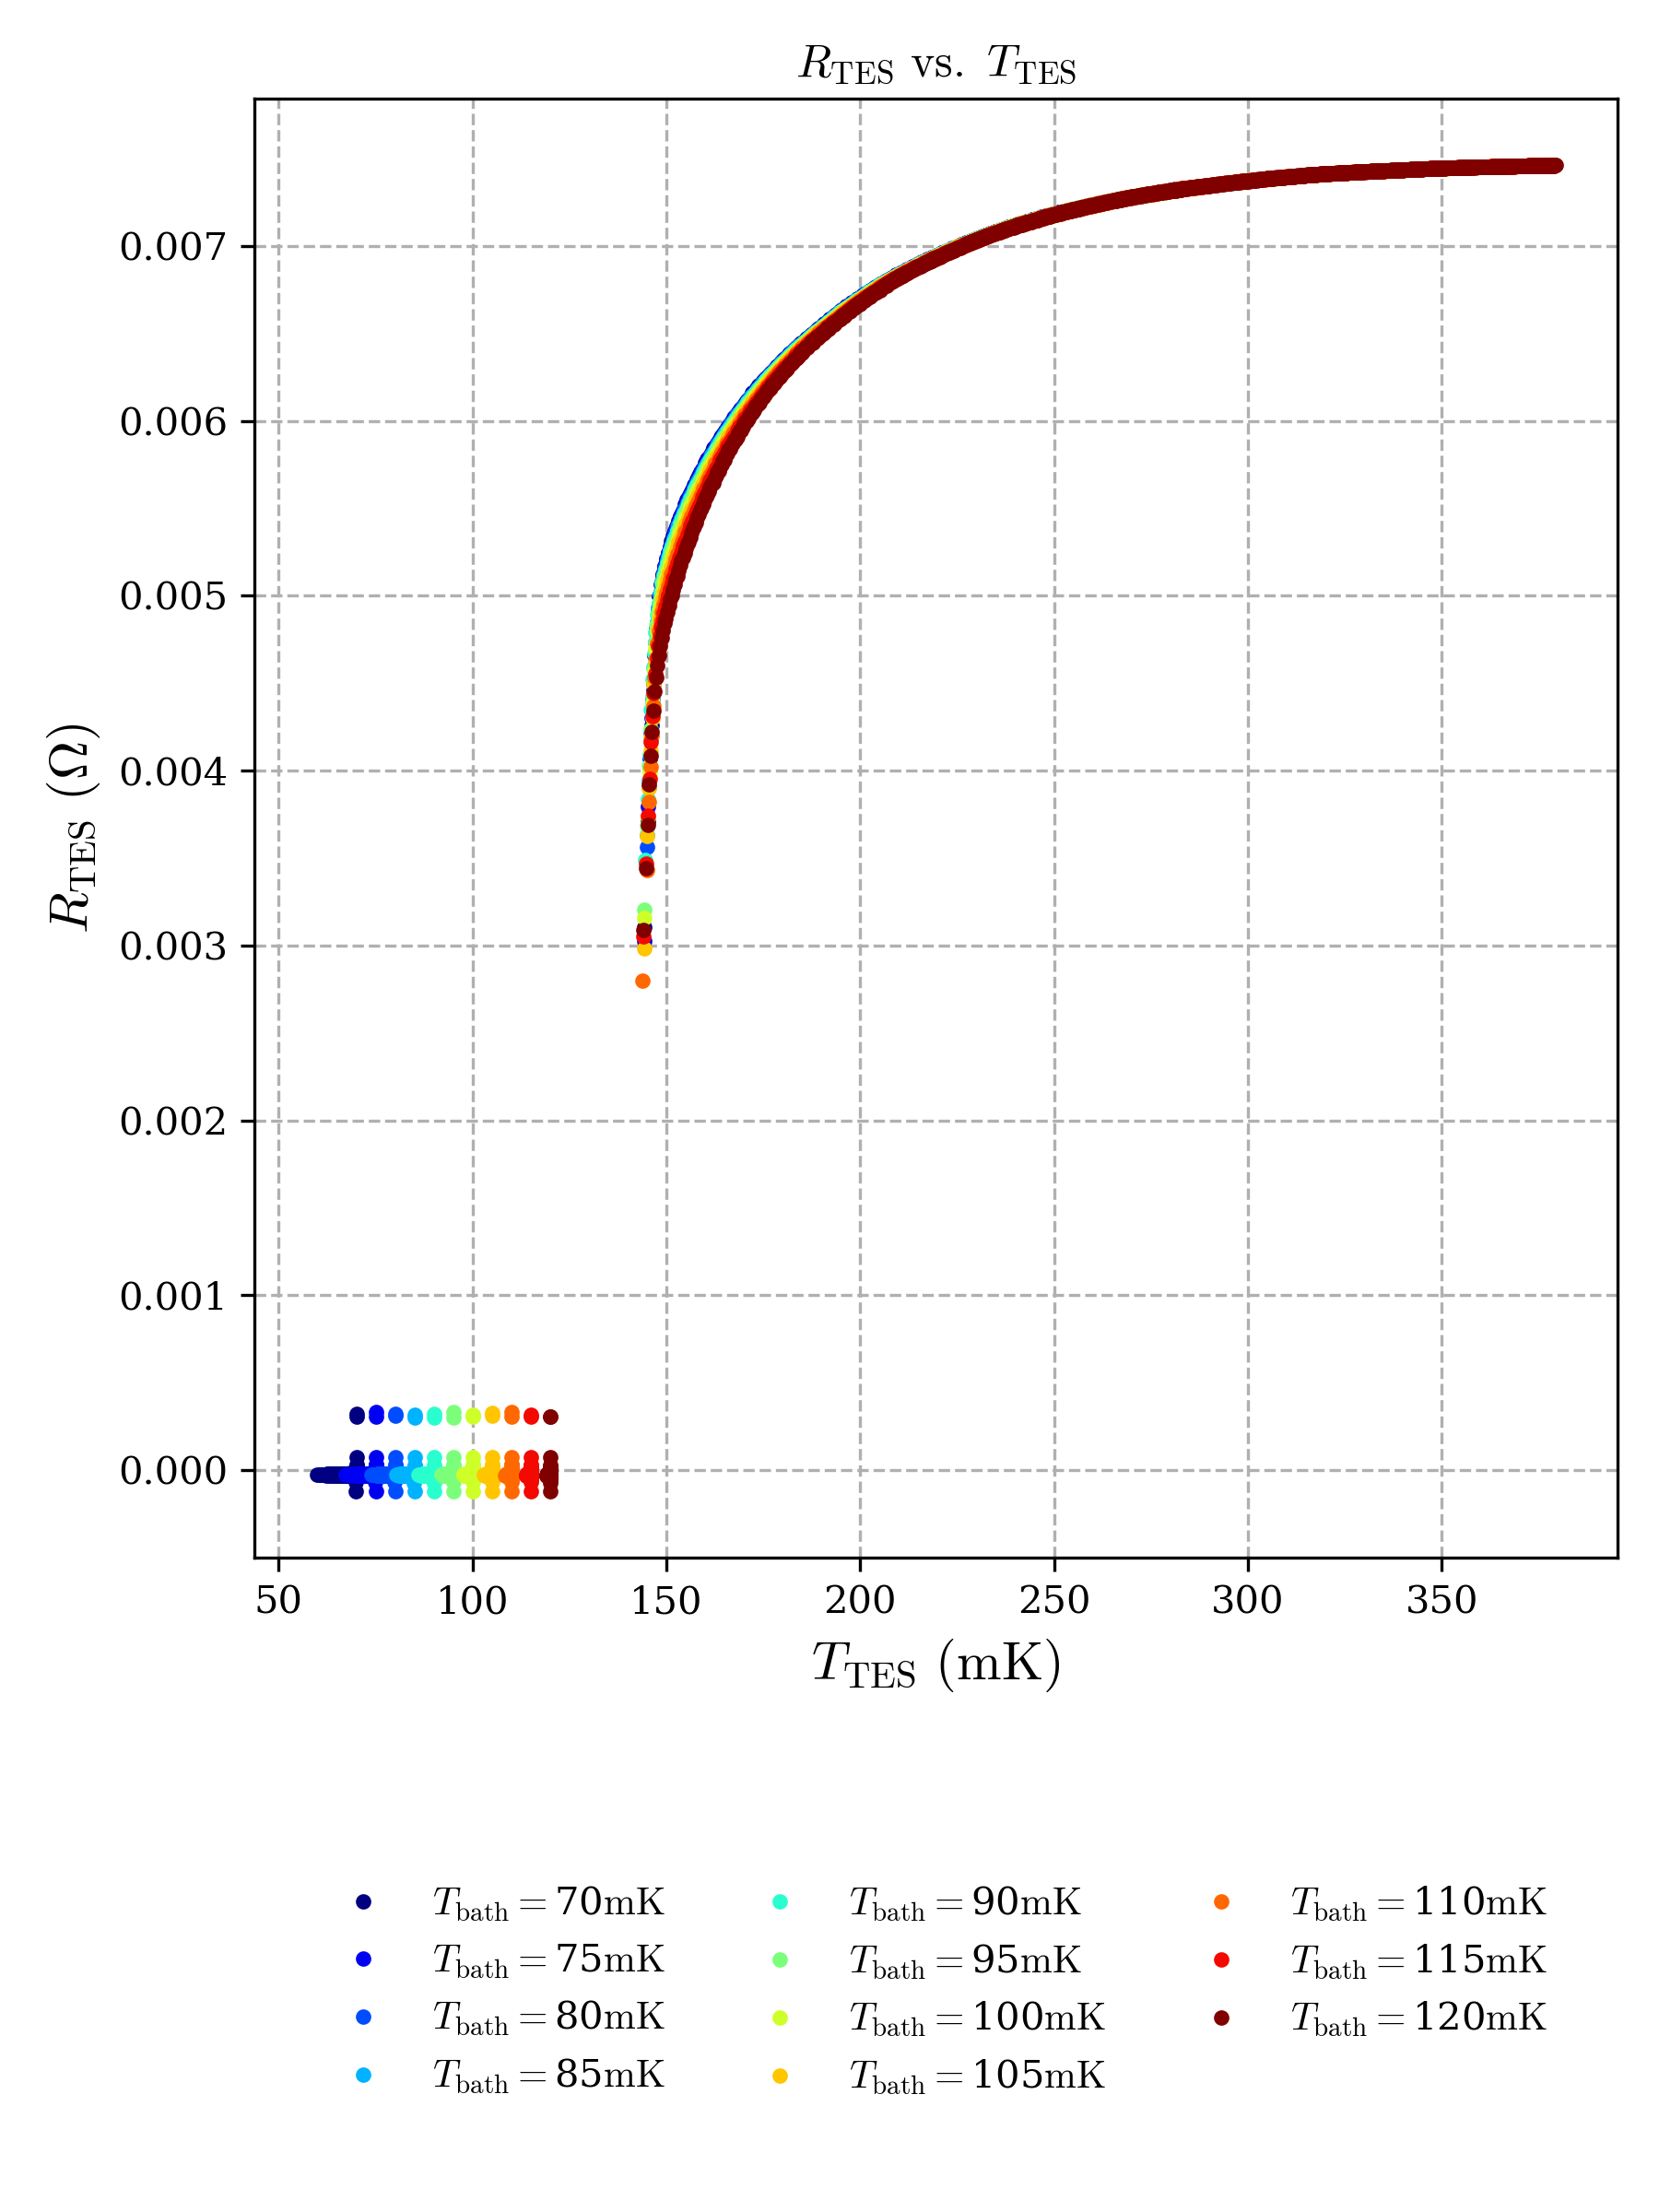
\includegraphics[width=0.8\textwidth]{IVtes_RTproperty.png}
    \label{fig:IVtesRTproperty}
\end{figure}
\clearpage

\subsection*{IVtes\_GTproperty}
TESの熱伝導度$G_{\rm TES }$とTESの温度$T_{\rm TES}$の関係
\[
G_{\rm TES} = G_0T_{\rm TES}^{n-1}
\]
をプロットする。$G_0$と$n$は,フィッティング結果の値を用いる。
\\ 図は$G_{\rm TES }$と$T_{\rm TES}$の関係をプロットしたものである。
\begin{figure}[H]
    \centering
    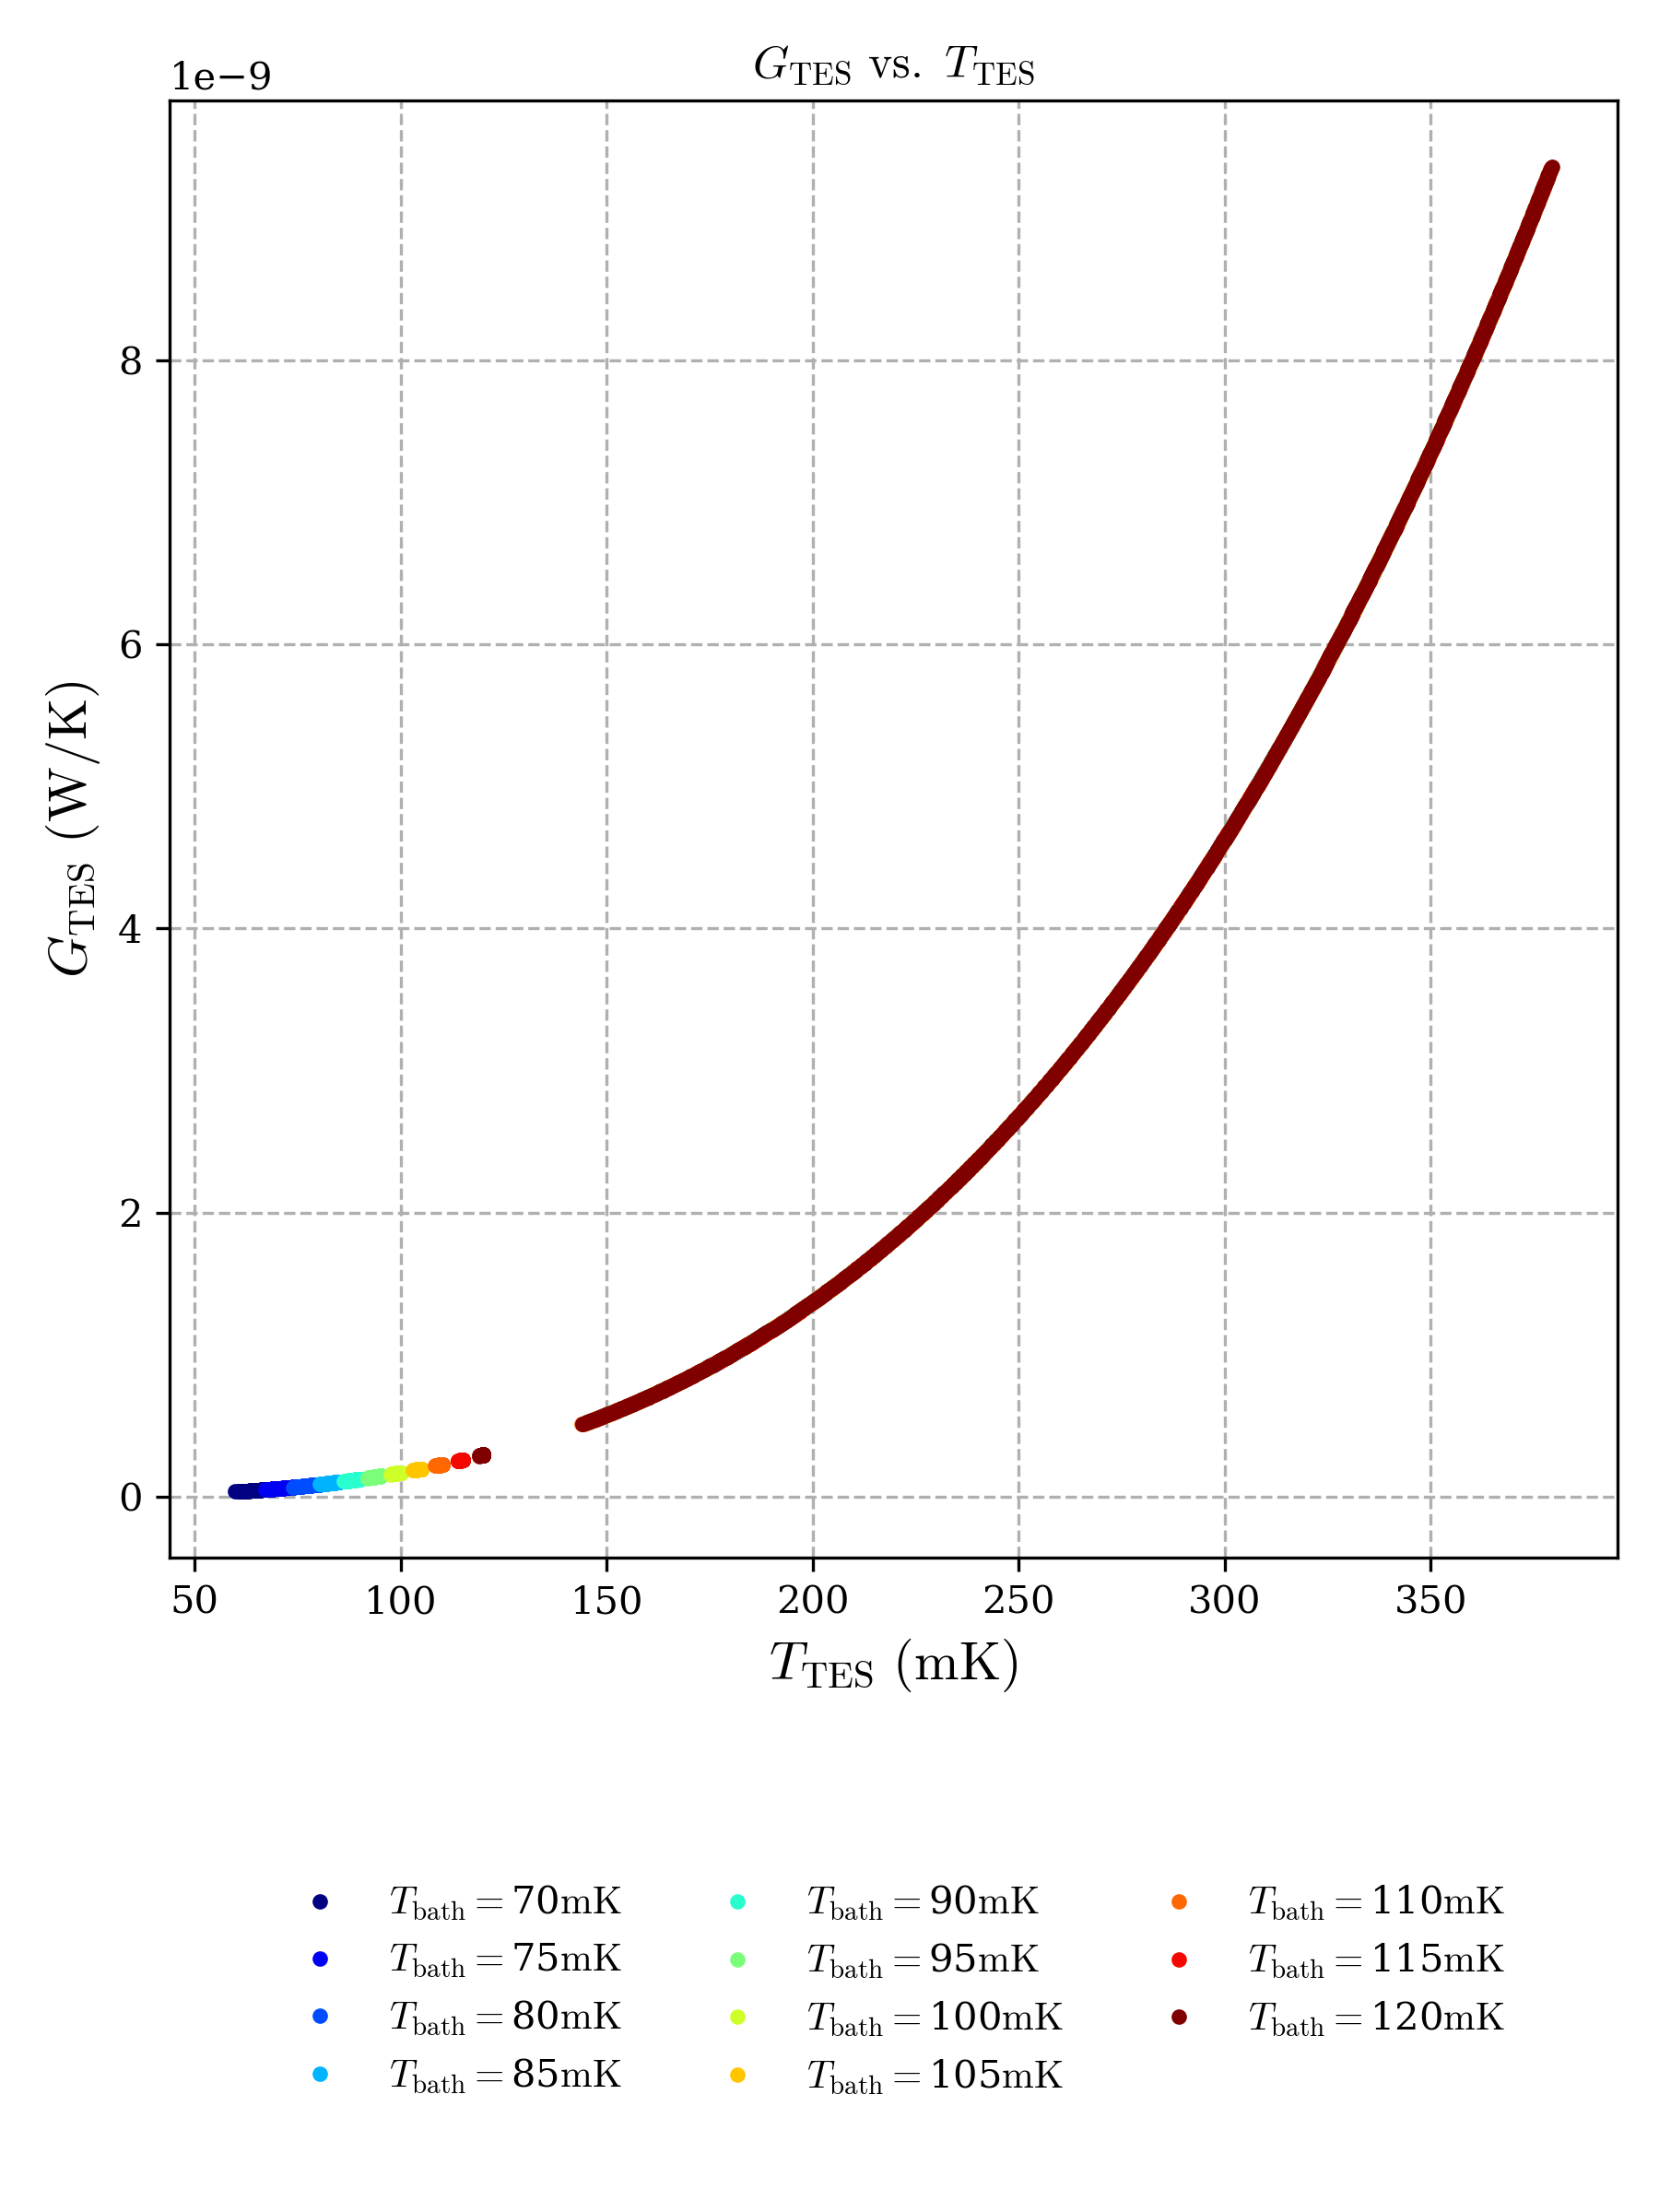
\includegraphics[width=0.8\textwidth]{IVtes_GTproperty.png}
    \label{fig:IVtesGTproperty}
\end{figure}
\clearpage

\subsection*{IVtes\_alpha}
TESの感度$\alpha$
\[
\alpha = \frac{T}{R}\frac{{\rm d}R}{{\rm d}T}
\]
をプロットする。TESの温度とTESの抵抗はともに$T_{\rm bath}=100\ {\rm mK}$のときの値を用いた。
\\ 図は$T_{\rm bath}=100\ {\rm mK}$のときの$\alpha$と$I_{\rm bias}$の関係をプロットしたものである。
\begin{figure}[H]
    \centering
    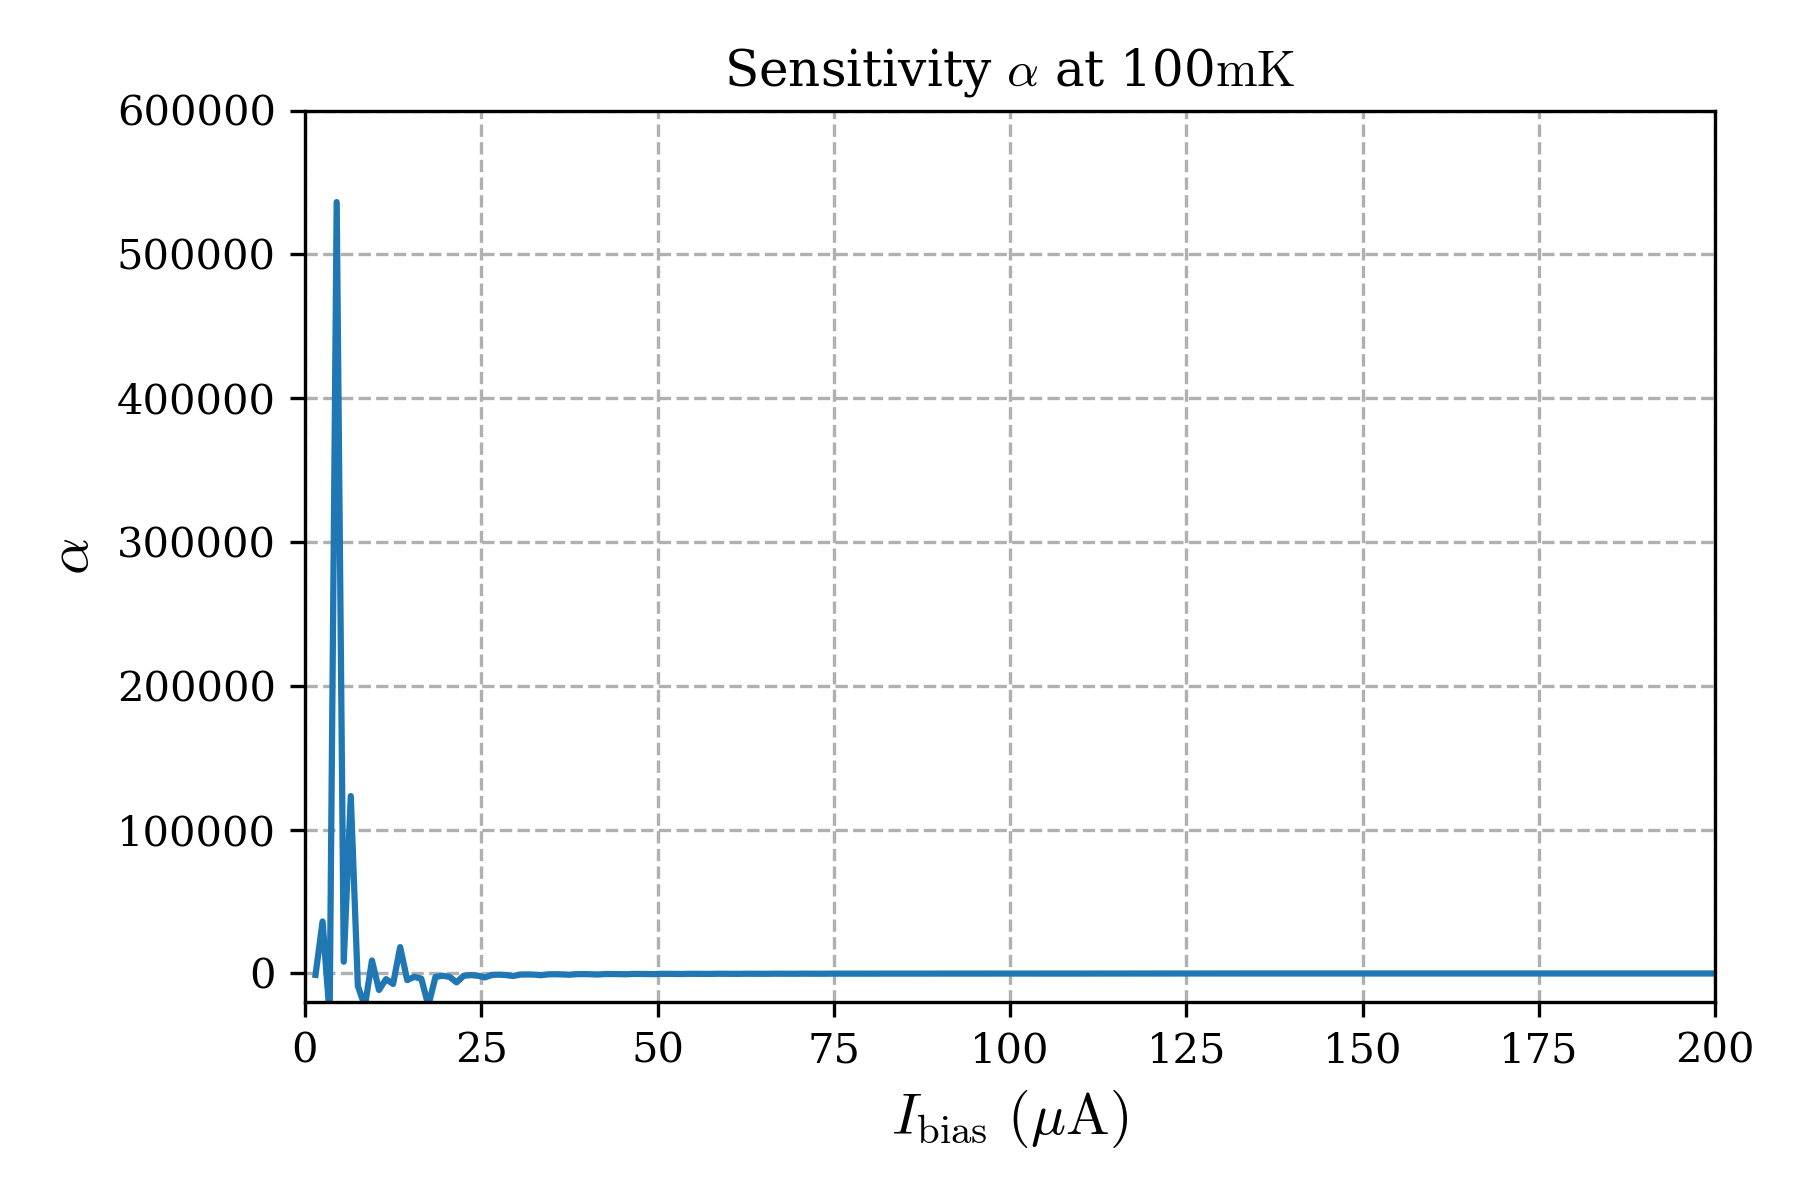
\includegraphics[width=0.8\textwidth]{IVtes_alpha.png}
    \label{fig:IVtesalpha}
\end{figure}
\clearpage

\subsection*{IVtes\_contour}
フィッティングパラメータのコントアをプロットする。信頼範囲の定義として,自由度2のカイ二乗分布における累積確率の値からパーセント点を求める。
累積確率は$68.27\ \%,\ 90\ \%,\ 99\ \%$の3点のP値を考えることとする。\\ 図は$n,\ G_0,\ T_{\rm c}$のそれぞれを2つのパラメータでコントアをプロットしたものである。
\begin{figure}[H]
    \centering
    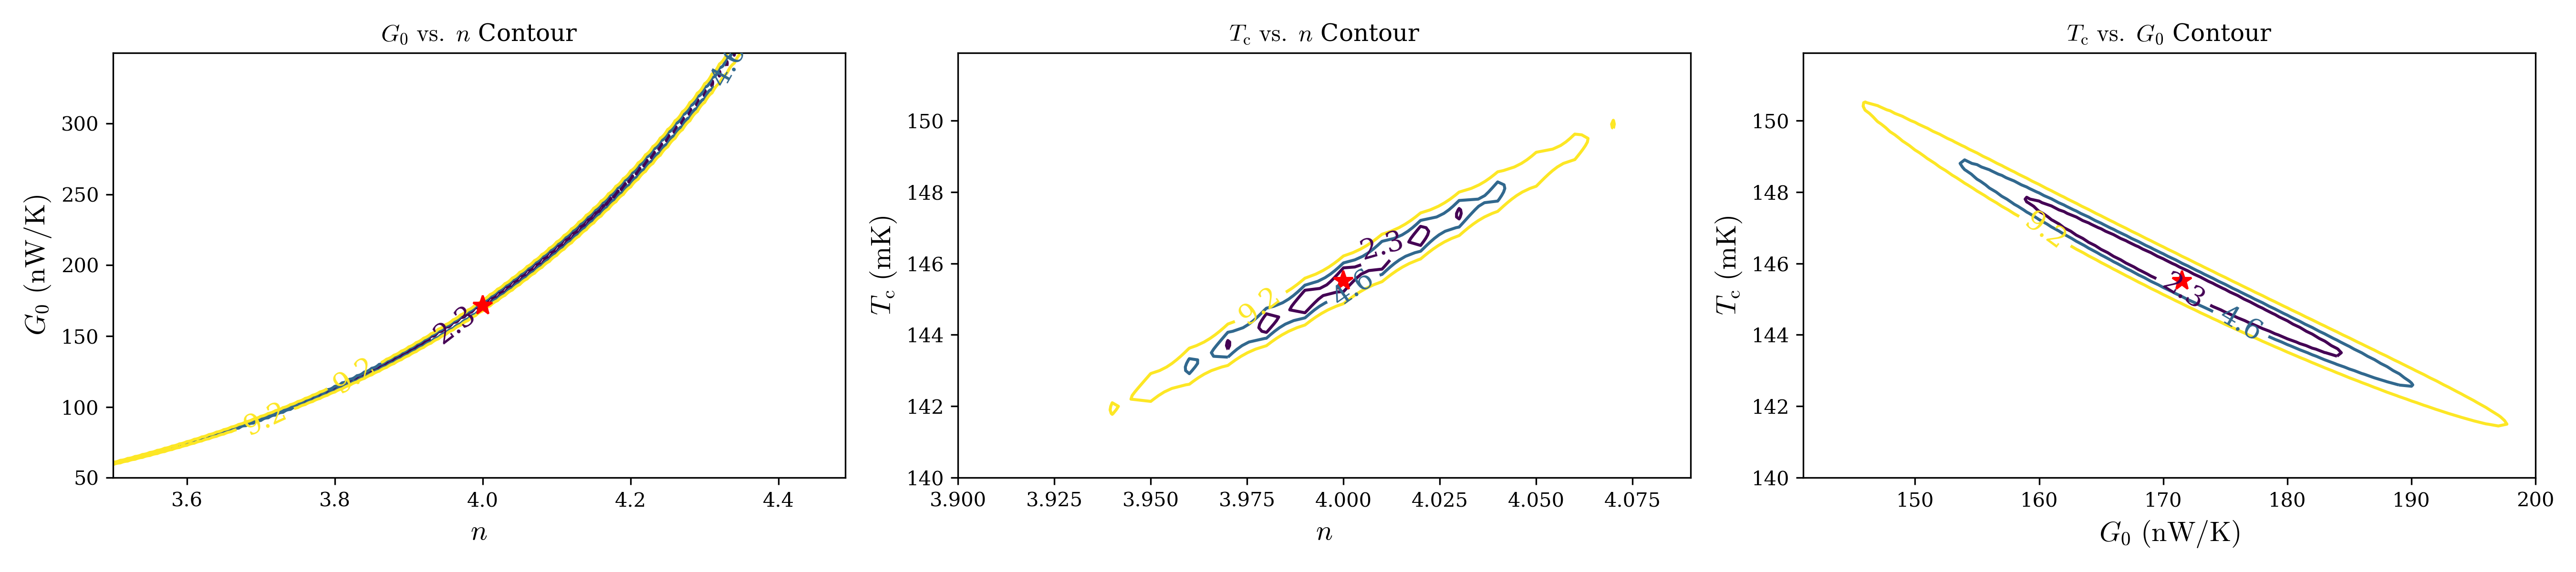
\includegraphics[width=0.8\textwidth]{IVtes_contour.png}
    \label{fig:IVtescontour}
\end{figure}

\end{document}
